\documentclass{article}
\usepackage[landscape]{geometry}
\usepackage{url}
\usepackage{multicol}
\usepackage{amsmath}
\usepackage{esint}
\usepackage{amsthm}
\usepackage{amsfonts}
\usepackage{booktabs}
\usepackage{tikz}
\usetikzlibrary{decorations.pathmorphing}
\usetikzlibrary{graphs}
\usetikzlibrary{shapes}
\usetikzlibrary{backgrounds}
\usetikzlibrary{calc}
\usetikzlibrary{patterns}
\usetikzlibrary{positioning, fit, arrows.meta}
\usepackage{amsmath,amssymb}
\usepackage{subcaption}
\usepackage[english]{babel}
\usepackage{enumitem}


\usepackage{colortbl}
\usepackage{xcolor}
\usepackage{mathtools}
\usepackage{amsmath,amssymb}
\usepackage{enumitem}
\makeatletter

\definecolor{horange}{HTML}{f58026}

\newcommand*\bigcdot{\mathpalette\bigcdot@{.5}}
\newcommand*\bigcdot@[2]{\mathbin{\vcenter{\hbox{\scalebox{#2}{\(\m@th#1\bullet\)}}}}}
\makeatother

\newenvironment{solution}%
    {\textit{Solution.}}

    \newcommand{\sol}[1]{
        \begin{solution}
            #1
        \end{solution}
    }

\title{Discrete Exam 2 Note Sheets}
\usepackage[utf8]{inputenc}

\advance\topmargin-.8in
\advance\textheight
3in
\advance\textwidth3in
\advance\oddsidemargin-1.40in
\advance\evensidemargin-1.45in
\parindent0pt
\parskip1pt
\newcommand{\hr}{\centerline{\rule{3.5in}{1pt}}}

% Natural Numbers 
\newcommand{\N}{\ensuremath{\mathbb{N}}}

% Whole Numbers
\newcommand{\W}{\ensuremath{\mathbb{W}}}

% Integers
\newcommand{\Z}{\ensuremath{\mathbb{Z}}}

% Rational Numbers
\newcommand{\Q}{\ensuremath{\mathbb{Q}}}

% Real Numbers
\newcommand{\R}{\ensuremath{\mathbb{R}}}

% Complex Numbers
\newcommand{\C}{\ensuremath{\mathbb{C}}}

\newcommand{\cyanit}[1]{\textbf{\textit{#1}}}

\newcommand{\brackett}[1]{\left\langle #1 \right\rangle}

\newcommand{\norm}[1]{\left\lVert \mathbf{#1}\right\rVert}

\newcommand{\dydx}{\tfrac{dy}{dx}}
\newcommand{\dxdy}{\tfrac{dx}{dy}}
\newcommand{\dydt}{\tfrac{dy}{dt}}
\newcommand{\dxdt}{\tfrac{dx}{dt}}
\newcommand{\dzdt}{\tfrac{dz}{dt}}


\newcommand{\cost}{\cos(t)}
\newcommand{\sint}{\sin(t)}
\newcommand{\tant}{\tan(t)}
\newcommand{\p}{\partial}

% 
\newcommand{\barNotationT}[1]{\bigg|_{t = #1}}

\newcommand{\mb}[1]{\mathbf{#1}}

\newcommand{\imb}{\mb{i}}
\newcommand{\jmb}{\mb{j}}
\newcommand{\kmb}{\mb{k}}
\newcommand{\rmb}{\mb{r}}
\newcommand{\umb}{\mb{u}}

\newcommand{\vecfuc}[2]{\mb{#1}(#2)}
\newcommand{\dvecfuc}[2]{\mb{#1}'(#2)}
\newcommand{\normdvecfuc}[2]{||\mb{#1}'(#2)||}

\DeclareMathOperator{\arccot}{arccot}
\DeclareMathOperator{\arcsec}{arcsec}
\DeclareMathOperator{\arccsc}{arccsc}

\usepackage{titlesec}

\newcommand{\mysqrt}[1]{%
  \mathpalette\foo{#1}%
}
\newcommand{\dmysqrt}[1]{%
  \mathpalette\foodisplay{#1}%
}

% !TeX spellcheck = off
\newcommand{\foo}[2]{%
  % #1: math style, #2: content
  \sbox0{$#1\sqrt{#2}$}% Measure the size of the standard sqrt in the current style
  \begin{tikzpicture}[baseline=(sqrt.base)]
    \node[inner sep=0, outer sep=0] (sqrt) {$#1\sqrt{#2}$}; % Use the current math style
    \draw([yshift=-0.045em]sqrt.north east) -- ++(0,-0.5ex); % Draw the tick
  \end{tikzpicture}%
}
% !TeX spellcheck = off
\newcommand{\foodisplay}[2]{%
  % #1: math style, #2: content
  \sbox0{$#1\sqrt{#2}$}% Measure the size of the standard sqrt in the current style
  \begin{tikzpicture}[baseline=(sqrt.base)]
    \node[inner sep=0, outer sep=0] (sqrt) {$\displaystyle\sqrt{#2}$}; % Force displaystyle
    \draw[line width=0.4pt] ([yshift=-0.044em]sqrt.north east) -- ++(0,-0.5ex); % Draw the tick
  \end{tikzpicture}%
}

\setlist[enumerate,1]{left=0pt}
\setlist[enumerate,2]{left=-10pt}


\begin{document}





















\begin{center}{\huge{\textbf{Multivariable Calculus Exam 2}}}\\
\end{center}
\begin{multicols*}{2}

    \tikzstyle{mybox} = [draw=black, fill=white, very thick,
    rectangle, rounded corners, inner sep=5pt, inner ysep=10pt]
    \tikzstyle{innerbox} = [draw=black, fill=gray!20, thick,
    rectangle, rounded corners, inner sep=5pt, inner ysep=10pt]
    \tikzstyle{fancytitle} =[fill=black, text=white, font=\bfseries]

    %------------ Measures of Center ---------------
    \begin{tikzpicture}
        \node [mybox] (box){%
            \begin{minipage}{0.46\textwidth}

                \begin{enumerate}
                    \item Show that \( \lim_{(x,y) \to (0,0)} \tfrac{xy^{2}}{x^{2}+y^{4}}\) does not exist.

                        \vspace*{-1em}
                        \begin{multicols}{2}
                            \begin{itemize}
                                \item \(x = 0 \) path: \( \lim_{(x,y) \to (0,0)} \tfrac{0 \cdot y^{2}}{0 + y^{4}} = \tfrac{0}{y^{2}} = 0\).
                                \item \(y = 0 \) path: \( \lim_{(x,y) \to (0,0)} \tfrac{x \cdot 0}{x^{2} + 0} = \tfrac{0}{x^{2}} = 0\).
                            \end{itemize}
                        \end{multicols}
                        \begin{itemize}
                            \item \(x = y^{2}\) path: \( \lim_{(x,y) \to (0,0)} \tfrac{y^{2} \cdot y^{2}}{y^{4} + y^{4}} = \tfrac{y^{4}}{2y^{4}} = \tfrac{1}{2}\).
                        \end{itemize}
                        Since the limit is not the same along all paths, the limit does not exist.

                        \item \(\tfrac{\p^{2}}{\p x \p y}\) \(\bigl(x^{3}y - y^{3}\tan(xy)\bigr)\) 
                        \vspace*{-1em}

                            \begin{align*}
                                \tfrac{\p^{2}}{\p x \p y} \bigl(x^{3}y - y^{3}\tan(xy)\bigr) &= \tfrac{\partial}{\partial x}\left[\tfrac{\partial}{\partial y}[x^{3}y] - \tfrac{\partial}{\partial y}\bigl[y^{3}\tan(xy)\bigr]\right] \\
                                &= \tfrac{\partial}{\partial x}\left[x^{3} - (3y^{2}\tan(xy) + xy^{3}\sec^{2}(xy))\right] \\
                                &= \tfrac{\partial}{\partial x}[x^{3}] - \tfrac{\partial}{\partial x}\bigl[3y^{2}\tan(xy)\bigr] - \tfrac{\partial}{\partial x}\bigl[xy^{3}\sec^{2}(xy)\bigr].
                            \end{align*}
                            Splitting this into 3 partial derivatives:
                            \[
                              \tfrac{\partial}{\partial x}[x^{3}] = 3x^{2}, \quad -\tfrac{\partial}{\partial x}\bigl[3y^{2}\tan(xy)\bigr] = -3y^{3}\sec^{2}(xy),
                            \]
                            with the final derivative worked out:
                            \begin{align*}
                                -\tfrac{\partial}{\partial x} \bigl[xy^{3}\sec^{2}(xy)\bigr] &= y^{3}\sec^{2}(xy) + \bigl[(xy^{3}) \cdot 2y\sec^{2}(xy)\tan(xy)\bigr] \\
                                &= -y^{3}\sec^{2}(xy) - 2xy^{4}\sec^{2}(xy)\tan(xy).
                            \end{align*}
                            Combining these results, we have:
                            \[
                              3x^{2} - 3y^{3}\sec^{2}(xy) - y^{3}\sec^{2}(xy) - 2xy^{4}\sec^{2}(xy)\tan(xy).
                            \]
                            Since three terms contain a factor of \(y^{3}\sec^{2}(xy)\), we can factor this out to get:
                            \[
                              3x^{2} - y^{3}\sec^{2}(xy)\bigl(3 + 1 + 2xy\tan(xy)\bigr).
                            \]
                            Adding and simplifying further, we get:
                            \[
                              \boxed{3x^{2} - 2y^{3}\sec^{2}(xy)\bigl(2 + xy\tan(xy)\bigr).} 
                            \] 
                            \item For the function \(f(x,y,z) = \dfrac{x + \sin(xy)}{x^{2} + y^{2} + z^{2} + 1}\), find \(\nabla f(x,y,z)\). \\
                            From the handout, we know that:
                            \[
                                \nabla f(x, y, z) = \dfrac{\partial f}{\partial x}(x, y, z)\mathbf{i} + \dfrac{\partial f}{\partial y}(x, y, z)\mathbf{j} + \dfrac{\partial f}{\partial z}(x, y, z)\mathbf{k}.
                            \]
                \end{enumerate} 
            \end{minipage}
        };
        %------------ Measures of Center Header ---------------------
        \node[fancytitle, right=10pt] at (box.north west) {Practice Set \# 3};
    \end{tikzpicture}




    %------------ Discrete Random Variable and Distributions ---------------
    \begin{tikzpicture}
        \node [mybox] (box){%
            \begin{minipage}{0.46\textwidth}
                \begin{multicols}{2}
                    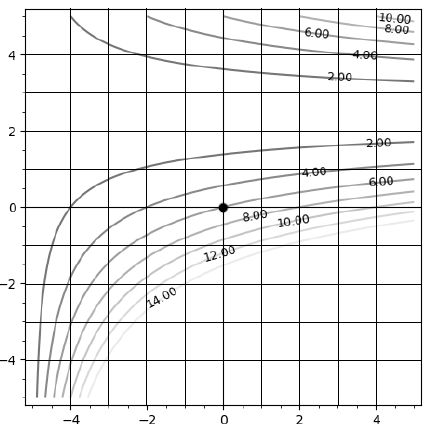
\includegraphics[width=6cm]{Images/contour_plot.png}
                    Determine the sign (\(+, \, -, \, 0\)) for each of the following partial derivatives.
                    \begin{enumerate}
                        \setcounter{enumi}{3}
                        \item \(f_{x}(0,0)\) \\
                            We see \(f(0,0) \approx 6\). Aswe move right (positive \(x\)), \(f\) increases, toward value 8. Thus, \(+\).
                        \item \(f_{y}(0,0)\) \\
                            As we move up \(f\) decreases twoard 4. Thus, \(-\).
                        \item \(f_{xx}(0,0)\) \\
                            The countours are evenly spread in the \(x\)-direction through \((0,0)\). We are increasing at a \underline{constant rate}. Hence, 0.
                        \item \(f_{yy}(0,0)\) \\
                            As we move in positive \(y\)-direction, we decrease, but less rapidly. The amount by which we are changing is \textit{increasing} (becoming less negative). Thus, \(+\). 
                        \item \(f_{xy}(0,0)\) \\
                            If we move in postive \(x\), the slope in the \(y\)-direction becomes more negative (i.e., decreases). Thus, \(-\).
                    \end{enumerate}
                \end{multicols}
                \begin{enumerate}
                    \setcounter{enumi}{8}
                    \item Find an equation of the tangent plane to \(f(x,y) = x^{2}y - \mysqrt{x} + y\) at the point \((3,1)\). \\
                    Solve for \(f_{x}(x,y)\), then \(f_{x}(3,1)\), and \(f_{y}(x,y)\), then \(f_{y}(3,1)\) to get the values of the partial derivatives at the point \((3,1)\):
                    \begin{align*}
                        z &= f(3,1) + f_{x}(3,1)(x - 3) + f_{y}(3,1)(y - 1) \\
                        &= 7 + \tfrac{23}{4}(x - 3) + \tfrac{35}{4}(y - 1)
                    \end{align*} 

                    \item Consider the function \(f(x,y) = x^{2}y - y^{3}\). Find the directional derivative for \(f\), at \((3,4)\), in the direction of \(\mb{u} = 5\imb - 2\jmb\). \\
                    Find 
                    \[
                    f_{x}(x,y) = 2xy, \quad f_{y}(x,y) = x^{2} - 3y^{2}.
                    \]
                    Then, at the point \((3,4)\):
                    \[
                    f_{x}(3,4) = 2 \cdot 3 \cdot 4 = 24, \quad f_{y}(3,4) = 3^{2} - 3 \cdot 4^{2} = -39.
                    \]
                    Then, we find the unit vector in the direction of \(\brackett{5,-2}\): 
                    \[
                    \tfrac{\brackett{24,-39} \cdot \brackett{5,-2}}{\mysqrt{29}} = \tfrac{198}{\mysqrt{29}}
                    \]
                \end{enumerate}
            \end{minipage}
        };
        %------------ Discrete Random Variable and Distributions Header ---------------------
        \node[fancytitle, right=10pt] at (box.north west) {Practice Set \# 3 (cont.)};
    \end{tikzpicture}

    %------------ Summarizing Main Features of f(x) ---------------
    \begin{tikzpicture}
        \node [mybox] (box){%
            \begin{minipage}{0.46\textwidth}
            \begin{enumerate}
                \item (3 points) Determine the absolute extrema for the function \(f(x,y) = x^{2} + 3y^{2} - 2x - y - xy\) on the triangular region with vertices \((0,0)\), \((2,0)\), and \((0,1)\). \\
          We first find the critical points of the function:
          \begin{align*}
            \nabla f(x,y) & = \langle 2x - 2 - y, \, 6y - 1 - x \rangle = \mathbf{0}  \\
            \implies y    & = 2x - 2 \quad \text{and} \quad x = 6(2x - 2) - 1 - x     \\
            \implies y    & = \tfrac{4}{11} \quad \text{and} \quad x = \tfrac{13}{11}
          \end{align*}
          This gives the critical point \(\boxed{\left(\frac{13}{11}, \frac{4}{11}\right)}\). We also need to check the boundary of the region. Thus:
          \begin{enumerate}[label=(\(\ell_{\arabic*}\)):]
            \item \(y = 0, \, 0 \leq x \leq 2 \implies f(x,y) = g(x) = x^{2} + 3(0)^{2} - 2x - (0) - x(0) = x^{2} - 2x \implies g'(x) = 2x - 2\). This gives \((1,0)\).
            \item \(x = 0, \, 0 \leq y \leq 1 \implies f(x,y) = h(y) = (0)^{2} + 3y^{2} - (0) - y - 0 = 3y^{2} - y \implies h'(y) = 6y - 1\). This gives \(\left(0, \frac{1}{6}\right)\)
            \item  \(y = 1 - \tfrac{1}{2}x, \, 0 \leq x \leq 2 \implies f(x,y) = k(x) = x^{2} + 3\left(1 - \tfrac{1}{2}x\right)^{2} - 2x - \left(1 -\tfrac{1}{2}x\right) - x\left(1 - \frac{1}{2}x\right).\)
                  \begin{align*}
                    k(x)           & = x^{2} + 3\left(1 - \tfrac{1}{2}x - \tfrac{1}{2}x + \tfrac{1}{4}x^{2}\right) - 2x - 1 + \tfrac{1}{2}x - x + \tfrac{1}{2}x^{2} \\
                                   & = \tfrac{1}{4}(9x^{2} - 22x + 8)                                                                                               \\
                    \implies k'(x) & = \tfrac{1}{4} \cdot \tfrac{d}{dx}[9x^{2} - 22x + 8]                                                                           \\
                    x              & = \tfrac{11}{9}
                  \end{align*}
                  Using this \(x\)-value, we plug it back into our equation for \(y\) to get the critical point \(\left(\frac{11}{9}, \frac{7}{18}\right)\).
          \end{enumerate}
          The vertices of the triangle give \(f(0,0) = 0\), \(f(2,0) = -2\), and \(f(0,1) = 2\). We can do the same for the other points and add them to our table.
          
          \begin{multicols}{2}
            \begin{center}
            \begin{tabular}{ccc}
              \toprule
              \textbf{Point} & \(f(x,y)\) & \textbf{Type} \\ \midrule
              \(\left(\tfrac{13}{11}, \tfrac{4}{11}\right)\) & \(-1.364\) & Interior CP \\ \midrule
              \((1,0)\) & \(-1\) & \(\ell_{1}\) \\ \midrule
              \(\left(0, \tfrac{1}{6}\right)\) & \(-0.083\) & \(\ell_{2}\) \\ \midrule
              \(\left(\tfrac{11}{9}, \tfrac{7}{18}\right)\) & \(\boxed{-1.361}\) & \(\ell_{3}\) \\ \midrule
              \((0,0)\) & \(0\) & Vertex 1 \\ \midrule
              \((2,0)\) & \(-2\) & Vertex 2 \\ \midrule
              \((0,1)\) & \(\boxed{2}\) & Vertex 3 \\ \bottomrule
            \end{tabular}
            \end{center}

            \flushright
            \begin{tikzpicture}[scale=1.5]
              \draw[->] (-0.5,0) -- (2.5,0) node[right] {\(x\)};
              \draw[->] (0,-0.5) -- (0,1.5) node[above] {\(y\)};
              \draw[color=horange, thick] (0,0) -- (2,0);
              \draw[color=horange, thick] (2,0) -- (0,1);
              \draw[color=horange, thick] (0,0)-- (0,1);
              \node[below left] at (0,0) {\(0\)};
              \node[below] at (2,0) {\(2\)};
              \node[left] at (0,1) {\(1\)};
              \node[below] at (1,0) {\(\ell_{1}\)};
              \node[left] at (0,0.5) {\(\ell_{2}\)};
              \node at (1,0.8) {\(\ell_{3}\)};
              \node[scale=0.7] at (13/11, 4/11) {\(\bullet\)};
              \node[scale=0.7] at (11/9, 7/18) {\(\bullet\)};
              \node[scale=0.7] at (0,1) {\(\bullet\)};
              \node[scale=0.7] at (0,0) {\(\bullet\)};
              \node[scale=0.7] at (2,0) {\(\bullet\)};
              \node[scale=0.7] at (0,1/6) {\(\bullet\)};
            \end{tikzpicture}
          \end{multicols}
        \end{enumerate}
            \end{minipage}
        };
        %------------ Summarizing Main Features of f(x) ---------------------
        \node[fancytitle, right=10pt] at (box.north west) {Practice Set \# 4};
    \end{tikzpicture}


    %------------ Sum and Average of Independent Random Variables ---------------
    \begin{tikzpicture}
        \node [mybox] (box){%
            \begin{minipage}{0.46\textwidth}
                \begin{enumerate}
                    \item Convert the rectangular point \((-5,1)\) to polar coordinates. \\
                      \begin{align*}
                        r & = \mysqrt{(-5)^{2} + 1^{2}} = \mysqrt{26} \\
                        \theta & = \arctan\left(\tfrac{1}{-5}\right) = \arctan\left(-\tfrac{1}{5}\right) = \tfrac{7\pi}{6} + \pi \text{ (2nd quadrant)}
                      \end{align*}
                      The polar coordinates are \(\boxed{\left(\mysqrt{26}, \tfrac{7\pi}{6} + \pi\right)}\).
                    \item Convert the cylindrical point \((5, \tfrac{7\pi}{6}, 2)\) to rectangular. \\
                      \begin{align*}
                        x & = 5\cos\left(\tfrac{7\pi}{6}\right) = 5\left(-\tfrac{\mysqrt{3}}{2}\right) = -\tfrac{5\mysqrt{3}}{2} \\
                        y & = 5\sin\left(\tfrac{7\pi}{6}\right) = 5\left(-\tfrac{1}{2}\right) = -\tfrac{5}{2} \\
                        z & = 2
                      \end{align*}
                      The rectangular coordinates are \(\boxed{\left(-\tfrac{5\mysqrt{3}}{2}, -\tfrac{5}{2}, 2\right)}\).
                    \item Convert the rectangular point \((-2,4,-1)\) to spherical.
                      \begin{align*}
                        \rho & = \mysqrt{(-2)^{2} + 4^{2} + (-1)^{2}} = \mysqrt{21} \\
                        \theta & = \arctan\left(\tfrac{4}{-2}\right) = \arctan\left(-2\right) \\
                        \phi & = \arccos\left(\tfrac{-1}{\mysqrt{21}}\right) = \arccos\left(-\tfrac{1}{\mysqrt{21}}\right)
                      \end{align*}
                      Since the point \((-2,4)\) is in the second quadrant, we add \(\pi\) to the arctan value. Hence, the spherical coordinates are \(\boxed{\left(\mysqrt{21}, \pi + \arctan\left(-2\right), \arccos\left(-\tfrac{1}{\mysqrt{21}}\right)\right)}\).
                    \item Convert the spherical point \((4, \frac{11\pi}{6}, \frac{3\pi}{4})\) to cylindrical. \\
                      The conversion from spherical to cylindrical follows the following equations:
                      \[
                        r = \rho \sin\phi, \quad \theta = \theta, \quad \text{and} \quad z = \rho \cos\phi.
                      \]
                      Thus, we have:
                      \begin{align*}
                        r & = 4\sin\left(\tfrac{3\pi}{4}\right) = 4\left(\tfrac{\mysqrt{2}}{2}\right) = 2\mysqrt{2} \\
                        \theta & = \tfrac{11\pi}{6} \\
                        z & = 4\cos\left(\tfrac{3\pi}{4}\right) = 4\left(-\tfrac{\mysqrt{2}}{2}\right) = -2\mysqrt{2}
                      \end{align*}
                      Therefore, we get the cylindrical coordinates \(\boxed{\left(2\mysqrt{2}, \tfrac{11\pi}{6}, -2\mysqrt{2}\right)}\).
                  \end{enumerate}
            \end{minipage}
        };
        %------------ Sum and Average of Independent Random Variables ---------------------
        \node[fancytitle, right=10pt] at (box.north west) {Practice Set \# 4 (cont.)};
    \end{tikzpicture}


    %------------ Maximum and Minimum of Independent Variables ---------------
    \begin{tikzpicture}
        \node [mybox] (box){%
            \begin{minipage}{0.46\textwidth}
        \begin{enumerate}
          \item \(\displaystyle\iint_{D}(x^{2} + 6xy) \, dA\) where \(D\) is the triangle with vertices \((0,0)\), \((4,0)\), and \((0,12)\) \\

          \sol{
            We can see that this triangle is bounded by three lines:
            \vspace*{-1.5em}
            \begin{center}
              \begin{minipage}{0.3\textwidth}
                \begin{tikzpicture}
                  \draw[->] (-0.25,0) -- (1.25,0) node[right] {\(x\)};
                  \draw[->] (0,-0.25) -- (0,3.25) node[above] {\(y\)};
                  \draw[color=horange, thick] (0,0) -- (1,0);
                  \draw[color=horange, thick] (1,0) -- (0,3);
                  \draw[color=horange, thick] (0,0) -- (0,3);
                  \node[below left] at (0,0) {\(0\)};
                  \node[below] at (1,0) {\(4\)};
                  \node[left] at (0,3) {\(12\)};
                  \node[below] at (1/2,0) {\(\ell_{1}\)};
                  \node[left] at (0,3/2) {\(\ell_{2}\)};
                  \node[right] at (1/2,3/2) {\(\ell_{3}\)};
                \end{tikzpicture}
              \end{minipage}%
              \begin{minipage}{0.3\textwidth}
                \begin{align*}
                  \ell_{1} & : y = 0 \\
                  \ell_{2} & : x = 0 \\
                  \ell_{3} & : y = -3x + 12
                \end{align*}
              \end{minipage}
            \end{center}
            \vspace*{-1em}
            This gives us the limits of integration as follows:
            \[
              \{(x,y) \colon 0 \leq x \leq 4, \quad 0 \leq y \leq -3x + 12\}.
            \]
            Thus, we can write the double integral as:
            \begin{align*}
              \iint_{D}(x^{2} + 6xy) \, dA & = \int_{0}^{4}\int_{0}^{-3x + 12}(x^{2} + 6xy) \, dy \, dx \\
              & = \int_{0}^{4}\left[x^{2}y + 3xy^{2}\right]_{0}^{-3x + 12} \, dx \\
              &= \int_{0}^{4}\left[x^{2}(-3x + 12) + 3x(-3x + 12)^{2}\right] \, dx \\
              &= 6\left[x^{4} - \tfrac{34}{3}x^{3} + 36x^{2}\right]_{0}^{4} \\
              &= 48\left[32 - \tfrac{34}{3}(8) + 36(2)\right] \\
              &= \boxed{640}
            \end{align*}
          }
                \end{enumerate}
            \end{minipage}
        };
        %------------ Maximum and Minimum of Independent Variables ---------------------
        \node[fancytitle, right=10pt] at (box.north west) {Practice Set \# 4 (cont.)};
    \end{tikzpicture}


    %------------ Some Continuous Distributions ---------------
    \begin{tikzpicture}
        \node [mybox] (box){%
            \begin{minipage}{0.46\textwidth}
              Suppose we have a general region \(D\). Then,
              \begin{itemize}
                \item \textbf{Type I Region} – we say that \(D\) is a Type I region provided there exists constants \(a\), \(b\) and continuous functions \(g_1\), \(g_2 : \R \to \R\) so that
                      \[
                        D = \{(x, y) : a \leq x \leq b, \text{ and } g_1(x) \leq y \leq g_2(x)\}.
                      \]
                \item \textbf{Type II Region} – we say that \(D\) is a Type II region provided there exists constants \(c\), \(d\) and continuous functions \(h_1\), \(h_2 : \R \to \R\) so that
                      \[
                        D = \{(x, y) : h_1(y) \leq x \leq h_2(y), \text{ and } c \leq y \leq d\}.
                      \]
              \end{itemize}
              \subsubsection{Type I Regions}
              
              Suppose that \(D\) is a type I region:
              \begin{align*}
                \iint_D f(x, y) \, dA & = \iint_R F(x, y) \, dA                             \\
                                      & = \int_b^a \int_{g_1(x)}^{g_2(x)} f(x, y) \, dy dx.
              \end{align*}
              The ``see below'' line is true since \(F(x, y) = 0\) if \(y > g_2(x)\) or \(y < g_1(x)\).
              
              \subsubsection{Type II Regions}
              
              In the same way, if \(D\) is type II, we have
              \[
                \iint_D f(x, y) \, dA = \int_d^c \int_{h_1(y)}^{h_2(y)} f(x, y) \, dx dy.
              \]
              How do you tell? DRAW A PICTURE! (In practice, you don’t typically explicitly note what type an integral is.)
              
              \subsubsection{Area}
              
              Suppose that \(D\) is a region. Then, the \cyanit{area} of \(D\) is given by
              \[
                \text{area}(D) = \iint_D 1 \, dA.
              \]
              
              \subsubsection{Average Value}
              
              The \cyanit{average value} of \(f\) over \(D\) is given by
              \[
                \text{ave}(f) = \frac{1}{\text{area}(D)} \iint_D f(x, y) \, dA.
              \]
            \end{minipage}
        };
        %------------ Some Continuous Distributions Header ---------------------
        \node[fancytitle, right=10pt] at (box.north west) {General Regions};
    \end{tikzpicture}


    %------------ Normal Distribution ---------------
    \begin{tikzpicture}
        \node [mybox] (box){%
            \begin{minipage}{0.46\textwidth}

              The statement that \((x_{0}, y_{0})\) is a \cyanit{critical point} of \(f\) means that either:
              \begin{itemize}
                  \item both \(f_{x}(x_{0}, y_{0}) = 0\) and \(f_{y}(x_{0}, y_{0}) = 0\), or
                  \item one or both partials does not exist.
              \end{itemize}
              
              \subsection{Maxima and Minima}
              
              \subsubsection{Local Extrema}
              
              The function \(f\) has a \cyanit{local maximum} at \((x_{0}, y_{0})\) provided that \(f(x_{0}, y_{0}) \geq f(x, y)\) for all choices of \((x, y)\) in some disk centered at \((x_{0}, y_{0})\) – that is, in some neighborhood of \((x_{0}, y_{0})\). \\
              
              Note that if there is a local extrema, \(\nabla f = \mb{0}\). This is because the gradient points in the direction of greatest increase, and if we are at a maximum or minimum, the function does not change. \\
              
              \subsubsection{Second Derivative Test}
              
              \textbf{Calculus I Version:} In Calculus I, the sign of the second derivative tells you whether a critical point is a local max/min, or inconclusive: Suppose that \(g \colon \R \to \R\) is a function of one variable, and \(x_{0}\) is a critical point.
              
              \begin{itemize}
                  \item if \(g''(x_{0}) > 0\), then \(x_{0}\) is a local minimum
                  \item if \(g''(x_{0}) < 0\), then \(x_{0}\) is a local maximum
                  \item if \(g''(x_{0}) = 0\), this test is inconclusive – it could be a max, min, or neither.
              \end{itemize}
              
              \textbf{Multivariable Calculus Version:} We have a similar test for \(f \colon \R^{2} \to \R\), where \((x_{0}, y_{0})\) is a critical point. Define
              \[
              D = f_{xx}(x_{0}, y_{0})f_{yy}(x_{0}, y_{0}) - (f_{xy}\bigl(x_{0}, y_{0})\bigr)^{2}.
              \]
              
              \begin{itemize}
                  \item if \(D > 0\) and \(f_{xx}(x_{0}, y_{0}) > 0\), then \(f\) has a local minimum
                  \item if \(D > 0\) and \(f_{xx}(x_{0}, y_{0}) < 0\), then \(f\) has a local maximum
                  \item if \(D < 0\), then \(f\) has a saddle point
                  \item if \(D = 0\), then the test is inconclusive
              \end{itemize}

            \end{minipage}
        };

        %------------ Normal Distribution Header ---------------------
        \node[fancytitle, right=10pt] at (box.north west) {Max and Min};
    \end{tikzpicture}
    %------------ Normal Distribution ---------------
    \begin{tikzpicture}
        \node [mybox] (box){%
            \begin{minipage}{0.46\textwidth}

              For functions \(f \colon \R^{2} \to \R\) we have a similar idea. If the surface generated by such a function has no sharp corners or edges, you might see that as you zoom in, the surface becomes flatter and flatter – and will eventually resemble a plane. In fact, we define the \cyanit{tangent plane} as the unique plane at \((x, y) = (x_{0}, y_{0})\) which satisfies
              \[
              z = f(x_{0}, y_{0}) + f_{x}(x_{0}, y_{0})(x - x_{0}) + f_{y}(x_{0}, y_{0})(y - y_{0}).
              \]
              
              Recall from Calculus I that if \(f\) is differentiable at \(x_{0}\) and \(x\) is close to \(x_{0}\) then
              \[
              f(x) \approx f(x_{0}) + f'(x_{0})(x - x_{0}).
              \]
              
              This is the \cyanit{linear approximation} of \(f\) at \(x_{0}\). In the same way, if \(f \colon \R^{2} \to \R\) is differentiable at \((x_{0}, y_{0})\) and \((x, y)\) is near \((x_{0}, y_{0})\), then
              \[
              f(x, y) \approx f(x_{0}, y_{0}) + f_{x}(x_{0}, y_{0})(x - x_{0}) + f_{y}(x_{0}, y_{0})(y - y_{0}).
              \]
              This is the \cyanit{linearization} of \(f\) at \((x_{0}, y_{0})\).
              
              \subsection{Examples}
              
              \(f(x,y) = x\cos(\pi x) \sin(\pi y)\), \((x_{0},y_{0}) = (\frac{1}{3}, \frac{1}{2})\). Our point of interest is \((\frac{1}{3}, \frac{1}{2}), \frac{1}{6}\), because we can just plug in the values of \(x_{0}\) and \(y_{0}\) into the function to get the height. \\
              
              To find the equation of the tangent plane, we need to find the partial derivatives to fill out the following equation:
              \[
              z = \underline{\hspace{1cm}} + \underline{\hspace{1cm}}\left(x - \frac{1}{3}\right) + \underline{\hspace{1cm}}\left(y - \frac{1}{2}\right).
              \]
              We found \(z_{0}\) to be \(\frac{1}{6}\), and the partial derivatives are
              \[
                  f_{x}(x,y) = \cos(\pi x)\sin(\pi y) - \pi x\sin(\pi x)\sin(\pi y),
              \]
              and 
              \[
                  f_{x}\left(\frac{1}{3},\frac{1}{2}\right) = \frac{1}{2} - \frac{\pi}{3}\left(\frac{\mysqrt{3}}{2}\right)(1) = \frac{1}{2} - \frac{\pi\mysqrt{3}}{3}.
              \]
              Similarly, we have
              \[
                  f_{y}\left(x,y\right) = \pi x\cos(\pi x)\cos(\pi y),
              \]
              and
              \[
                  f_{y}\left(\frac{1}{3},\frac{1}{2}\right) = 0.
              \]
              Now, we can fill out the rest of our equation:
              \[
              z = \frac{1}{6} + \left(\frac{1}{2} - \frac{\pi\mysqrt{3}}{3}\right)\left(x - \frac{1}{3}\right) + 0\left(y - \frac{1}{2}\right).
              \]
            \end{minipage}
        };

        %------------ Normal Distribution Header ---------------------
        \node[fancytitle, right=10pt] at (box.north west) {Tangent Planes};
    \end{tikzpicture}

\end{multicols*}



\end{document}